% Options for packages loaded elsewhere
\PassOptionsToPackage{unicode}{hyperref}
\PassOptionsToPackage{hyphens}{url}
%
\documentclass[
  ignorenonframetext,
  aspectratio=1610,
]{beamer}
\usepackage{pgfpages}
\setbeamertemplate{caption}[numbered]
\setbeamertemplate{caption label separator}{: }
\setbeamercolor{caption name}{fg=normal text.fg}
\beamertemplatenavigationsymbolsempty
% Prevent slide breaks in the middle of a paragraph
\widowpenalties 1 10000
\raggedbottom
\setbeamertemplate{part page}{
  \centering
  \begin{beamercolorbox}[sep=16pt,center]{part title}
    \usebeamerfont{part title}\insertpart\par
  \end{beamercolorbox}
}
\setbeamertemplate{section page}{
  \centering
  \begin{beamercolorbox}[sep=12pt,center]{part title}
    \usebeamerfont{section title}\insertsection\par
  \end{beamercolorbox}
}
\setbeamertemplate{subsection page}{
  \centering
  \begin{beamercolorbox}[sep=8pt,center]{part title}
    \usebeamerfont{subsection title}\insertsubsection\par
  \end{beamercolorbox}
}
\AtBeginPart{
  \frame{\partpage}
}
\AtBeginSection{
  \ifbibliography
  \else
    \frame{\sectionpage}
  \fi
}
\AtBeginSubsection{
  \frame{\subsectionpage}
}
\usepackage{amsmath,amssymb}
\usepackage{iftex}
\ifPDFTeX
  \usepackage[T1]{fontenc}
  \usepackage[utf8]{inputenc}
  \usepackage{textcomp} % provide euro and other symbols
\else % if luatex or xetex
  \usepackage{unicode-math} % this also loads fontspec
  \defaultfontfeatures{Scale=MatchLowercase}
  \defaultfontfeatures[\rmfamily]{Ligatures=TeX,Scale=1}
\fi
\usepackage{lmodern}
\ifPDFTeX\else
  % xetex/luatex font selection
\fi
% Use upquote if available, for straight quotes in verbatim environments
\IfFileExists{upquote.sty}{\usepackage{upquote}}{}
\IfFileExists{microtype.sty}{% use microtype if available
  \usepackage[]{microtype}
  \UseMicrotypeSet[protrusion]{basicmath} % disable protrusion for tt fonts
}{}
\makeatletter
\@ifundefined{KOMAClassName}{% if non-KOMA class
  \IfFileExists{parskip.sty}{%
    \usepackage{parskip}
  }{% else
    \setlength{\parindent}{0pt}
    \setlength{\parskip}{6pt plus 2pt minus 1pt}}
}{% if KOMA class
  \KOMAoptions{parskip=half}}
\makeatother
\usepackage{xcolor}
\newif\ifbibliography
\usepackage{graphicx}
\makeatletter
\def\maxwidth{\ifdim\Gin@nat@width>\linewidth\linewidth\else\Gin@nat@width\fi}
\def\maxheight{\ifdim\Gin@nat@height>\textheight\textheight\else\Gin@nat@height\fi}
\makeatother
% Scale images if necessary, so that they will not overflow the page
% margins by default, and it is still possible to overwrite the defaults
% using explicit options in \includegraphics[width, height, ...]{}
\setkeys{Gin}{width=\maxwidth,height=\maxheight,keepaspectratio}
% Set default figure placement to htbp
\makeatletter
\def\fps@figure{htbp}
\makeatother
\setlength{\emergencystretch}{3em} % prevent overfull lines
\providecommand{\tightlist}{%
  \setlength{\itemsep}{0pt}\setlength{\parskip}{0pt}}
\setcounter{secnumdepth}{-\maxdimen} % remove section numbering
\usepackage{pgfpages}
\usepackage{microtype}
\usepackage{tikz}
  \usetikzlibrary{positioning}
  \usetikzlibrary{arrows}
  \usetikzlibrary{graphs}

\definecolor{CTred}{RGB}{229,32,32}
\definecolor{CTgrey}{RGB}{153,153,153}

\usepackage{array}
\usepackage{dcolumn}
\newcolumntype{d}{D{.}{.}{-1}}
\usepackage{booktabs}
\usepackage{threeparttable}

% colors: white text on 90% black background
\setbeamercolor{normal text}{fg=black,bg=white}

% light blue as a highlight color
\setbeamercolor*{structure}{fg=CTred}
\setbeamercolor{section title}{fg=CTred}
\setbeamercolor{alerted text}{use=structure,fg=CTred}
\setbeamercolor*{palette primary}{use=structure,fg=structure.fg}
\setbeamercolor*{palette secondary}{use=structure,fg=structure.fg!95!black}
\setbeamercolor*{palette tertiary}{use=structure,fg=structure.fg!90!black}
\setbeamercolor*{palette quaternary}{use=structure,fg=structure.fg!95!black,bg=black!80}

\setbeamercolor*{framesubtitle}{fg=white}


% use system fonts: here, Gill Sans
\usefonttheme{professionalfonts}
\setbeamerfont{quote}{shape=\upshape}

% eliminate silly beamer navigation line at bottom of slides
\setbeamertemplate{navigation symbols}{}
\setbeamertemplate{footline}[frame number]

% ensure text jusfication
\usepackage{ragged2e}
\justifying

% pandoc makes 2nd-lever headers into blocks, and this ensures justification
% in blocks too
\addtobeamertemplate{block begin}{}{\justifying}




\urlstyle{same}
\usepackage[overlay,absolute]{textpos}

\setbeamertemplate{items}[square]

\TPGrid[10 mm,8 mm]{9}{8}
% beamer's left and right margin is 10 mm. The top/bottom margin is ??
% or without a header ??
% the slide dimensions are 128 mm x 96 mm
% so the resulting \TPHorizModule = 12 mm and \TPVertModule = 10 mm

% uncomment if you want biblatex for citations on slides

% \usepackage{csquotes}
% \usepackage[notes,short,noibid,backend=biber]{biblatex-chicago}
% \bibliography{course.bib} 

\providecommand{\exhibit}[2]{\includegraphics[keepaspectratio, height=0.9\textheight, width=\textwidth]{assets/img/#1}\\ {\tiny #2}}

\providecommand{\smallcite}[1]{({\footnotesize #1})}
\ifLuaTeX
  \usepackage{selnolig}  % disable illegal ligatures
\fi
\IfFileExists{bookmark.sty}{\usepackage{bookmark}}{\usepackage{hyperref}}
\IfFileExists{xurl.sty}{\usepackage{xurl}}{} % add URL line breaks if available
\urlstyle{same}
\hypersetup{
  pdftitle={Communist Era Managers in Modern Times: A Comparison of Management Skills Across Generations},
  pdfauthor={Miklós Koren (CEU, HUN-REN KRTK, CEPR and CESifo); Gergely Attila Kiss (HUN-REN KRTK, CEU and KSH)},
  hidelinks,
  pdfcreator={LaTeX via pandoc}}

\title{Communist Era Managers in Modern Times: A Comparison of
Management Skills Across Generations}
\author{Miklós Koren (CEU, HUN-REN KRTK, CEPR and CESifo) \and Gergely
Attila Kiss (HUN-REN KRTK, CEU and KSH)}
\date{March 21, 2024\footnote<.->{Supported by Forefront Research
  Excellence Grant (144193), and the European Research Council (313164
  and 101097789)}}

\begin{document}
\frame{\titlepage}

\section{Introduction}\label{introduction}

\begin{frame}{Hungary, 1980 (Fortepan / Szalay Zoltán)}
\protect\hypertarget{hungary-1980-fortepan-szalay-zoltuxe1n}{}
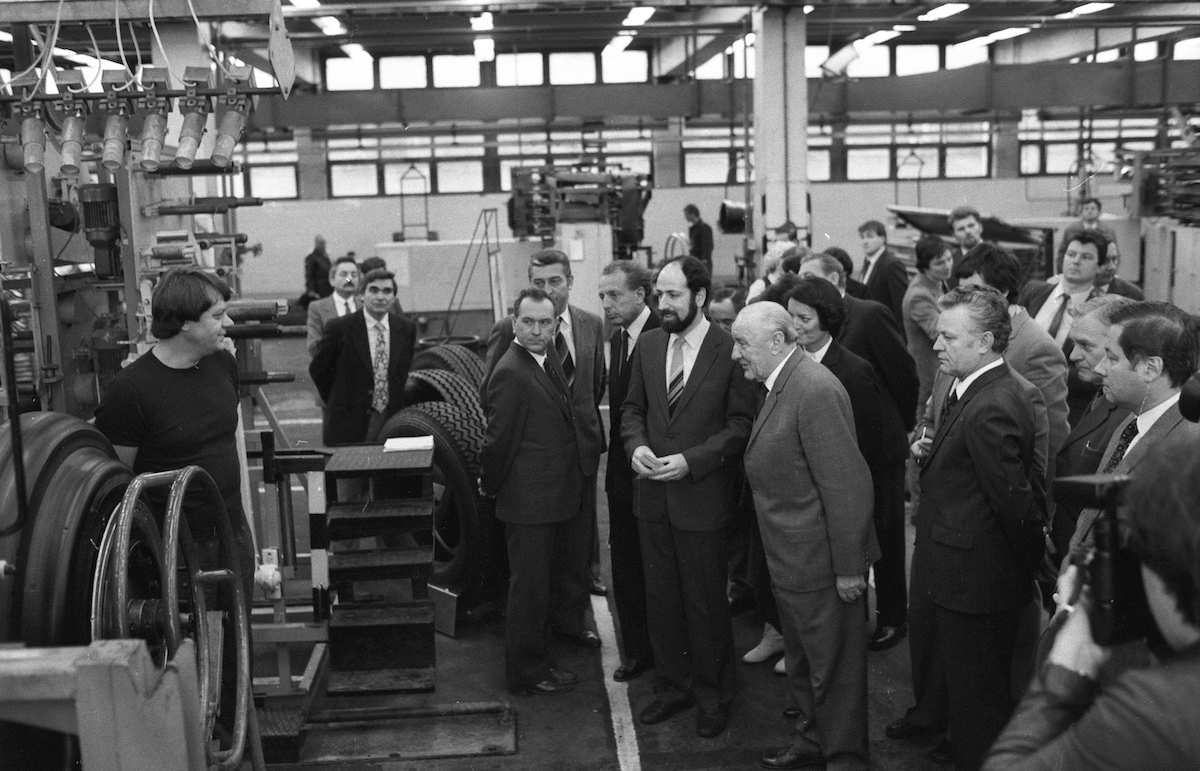
\includegraphics{fig/fortepan_198036.jpg}
\end{frame}

\begin{frame}{Hungary, 1990 (MTI)}
\protect\hypertarget{hungary-1990-mti}{}
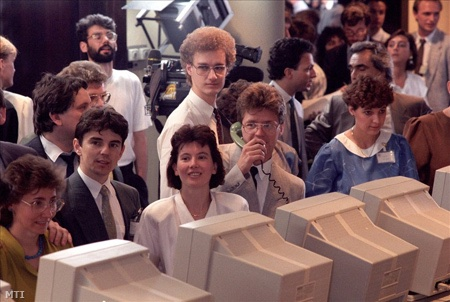
\includegraphics{fig/tozsde.jpg}
\end{frame}

\begin{frame}{Number of Executive Positions Increased}
\protect\hypertarget{number-of-executive-positions-increased}{}
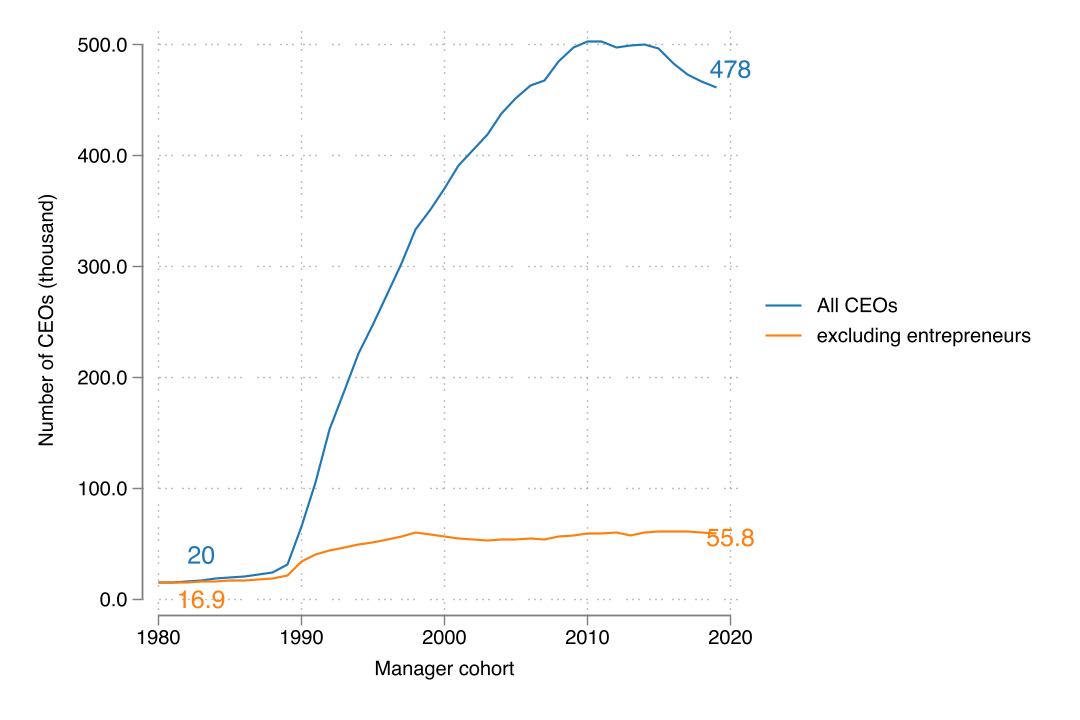
\includegraphics{fig/ceo-stock.png}
\end{frame}

\begin{frame}{Business Degrees Became More Prominent}
\protect\hypertarget{business-degrees-became-more-prominent}{}
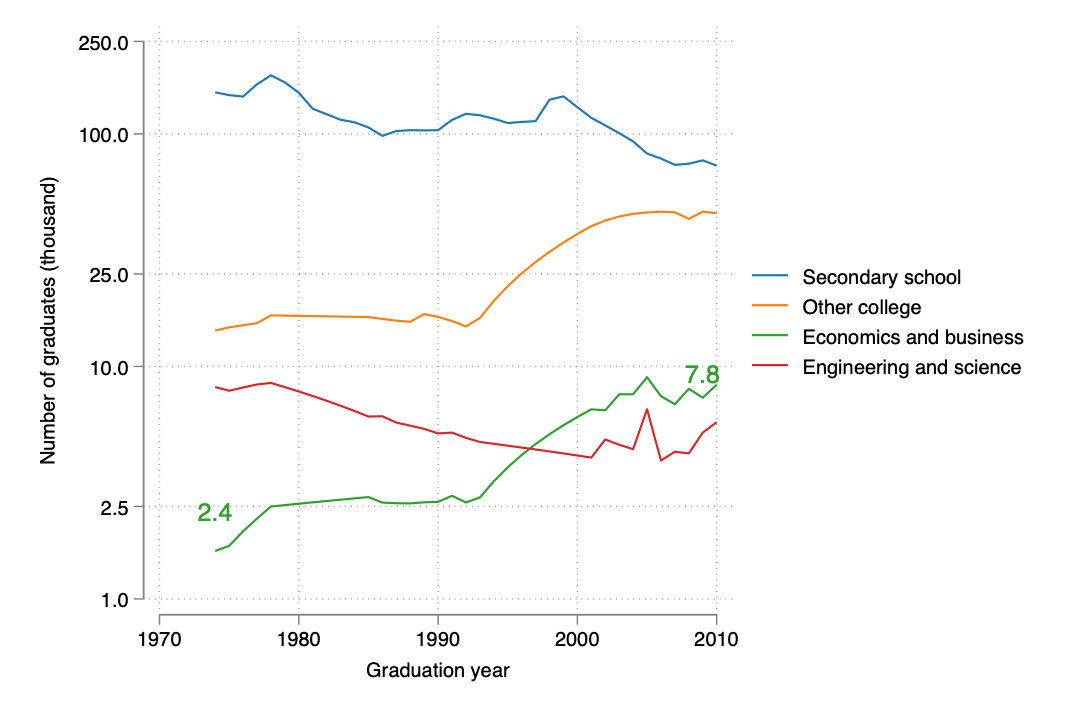
\includegraphics{fig/school-graduates.png}
\end{frame}

\begin{frame}{Why Micro \(\neq\) Macro}
\protect\hypertarget{why-micro-neq-macro}{}
\begin{block}{What we know}
\protect\hypertarget{what-we-know}{}
\begin{enumerate}
\tightlist
\item
  Management matters
\item
  Training works
\item
  Managers matter
\end{enumerate}

\pause
\end{block}

\begin{block}{What we don't know}
\protect\hypertarget{what-we-dont-know}{}
\begin{enumerate}
\tightlist
\item
  What policy interventions can improve management for an entire
  country?
\item
  How to quantify the macro effects of these policies?
\end{enumerate}

\pause
\end{block}

\begin{block}{What we need}
\protect\hypertarget{what-we-need}{}
\begin{enumerate}
\tightlist
\item
  Endogenous supply: how to incentivize people to become managers?
\item
  Selection: who will become managers?
\item
  Competition: what are the GE feedbacks of interventions?
\end{enumerate}
\end{block}
\end{frame}

\section{Setup and Data}\label{setup-and-data}

\begin{frame}{Data}
\protect\hypertarget{data}{}
\begin{block}{Manager Data 1985-2019}
\protect\hypertarget{manager-data-1985-2019}{}
Universe of corporations (1m) and their CEOs (1.3m). Firm size
(employment) as proxy for manager quality.
\end{block}

\begin{block}{Biographies}
\protect\hypertarget{biographies}{}
Full biographies (school, work experience, etc.) for 63k people in 2013.
30k matched to CEO panel.
\end{block}

\begin{block}{College graduates}
\protect\hypertarget{college-graduates}{}
Number of gradues by degree and year.
\end{block}
\end{frame}

\section{World Management Survey}\label{world-management-survey}

\begin{frame}{Methodology}
\protect\hypertarget{methodology}{}
\end{frame}

\begin{frame}{Hungarian wave}
\protect\hypertarget{hungarian-wave}{}
Spring and Summer of 2018.

Target population: manufacturing firms with 50+ employees.

Sample: 762 firms.
\end{frame}

\begin{frame}{Survey logistics}
\protect\hypertarget{survey-logistics}{}
10 surveyors

\begin{block}{Funnel}
\protect\hypertarget{funnel}{}
\begin{enumerate}
\tightlist
\item
  762 firms contacted by phone
\item
  281 (37\%) resulted in direct contact to manager
\item
  144 (51\%) scheduled an interview
\item
  126 (87\%) completed the interview
\item
  118 (94\%) usable responses
\end{enumerate}
\end{block}
\end{frame}

\section{Validation}\label{validation}

\begin{frame}{How old is your firm?}
\protect\hypertarget{how-old-is-your-firm}{}
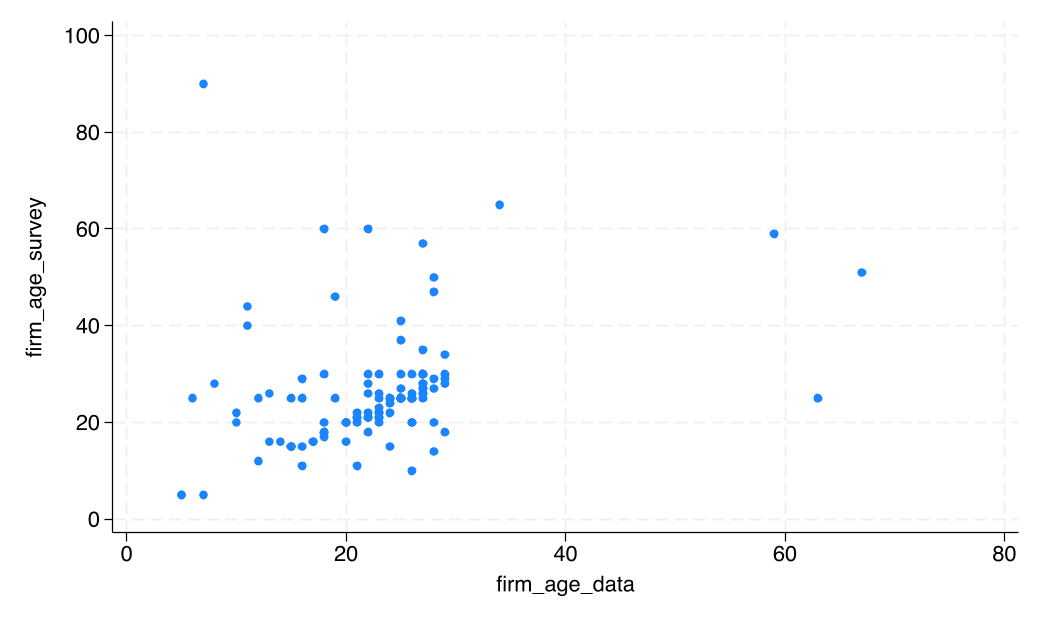
\includegraphics{fig/firm_age_validation.png}
\end{frame}

\begin{frame}{How many employees does your firm have?}
\protect\hypertarget{how-many-employees-does-your-firm-have}{}
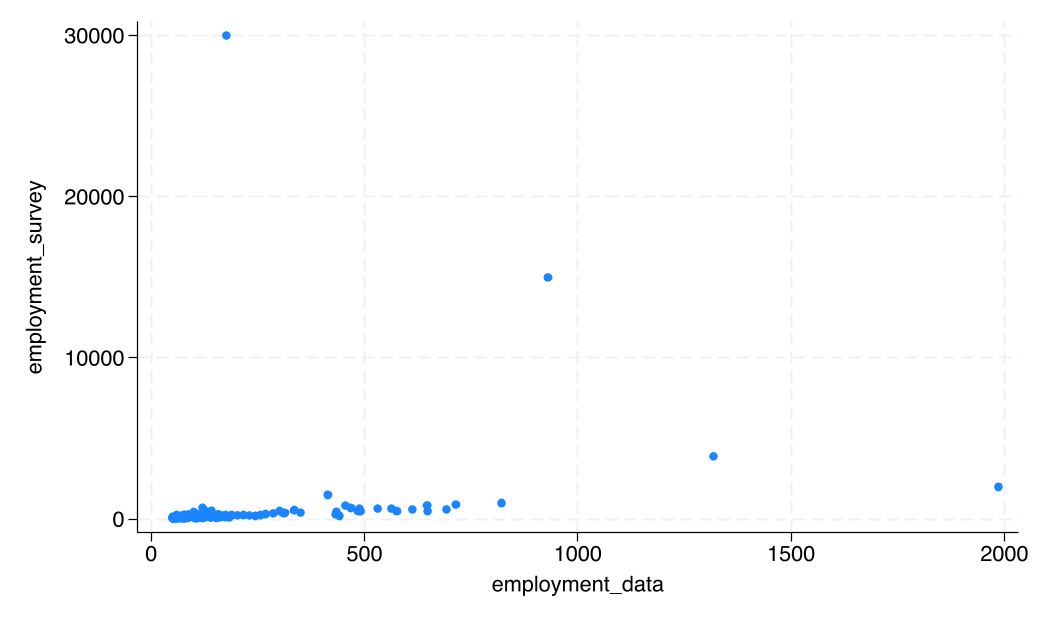
\includegraphics{fig/employment_validation.png}
\end{frame}

\begin{frame}{\ldots zooming in}
\protect\hypertarget{zooming-in}{}
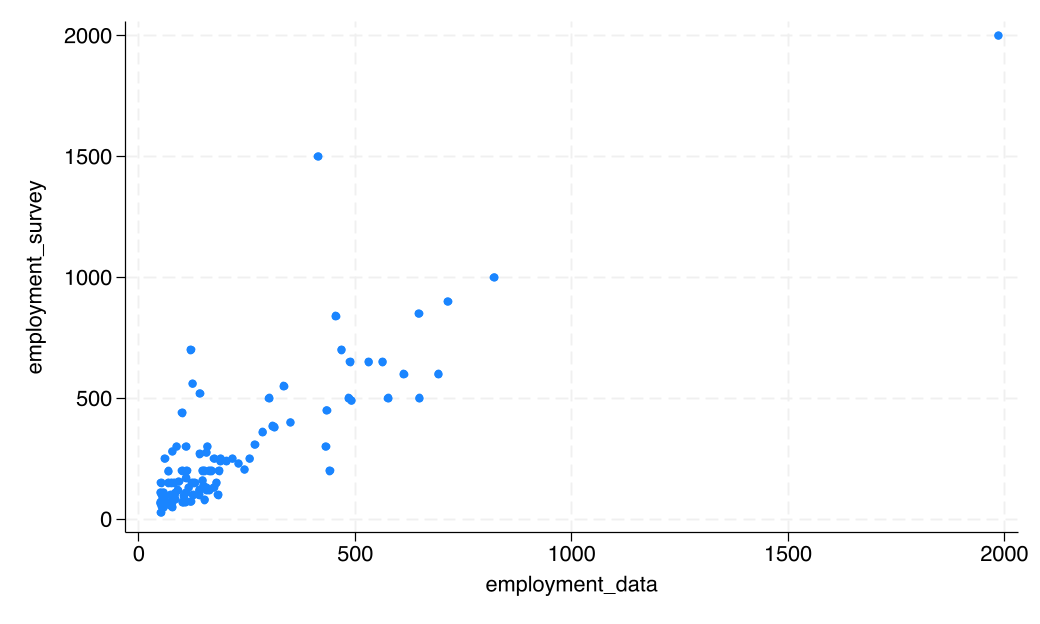
\includegraphics{fig/employment_validation_cleaned.png}
\end{frame}

\begin{frame}{What percentage of your revenue is coming from exports?}
\protect\hypertarget{what-percentage-of-your-revenue-is-coming-from-exports}{}
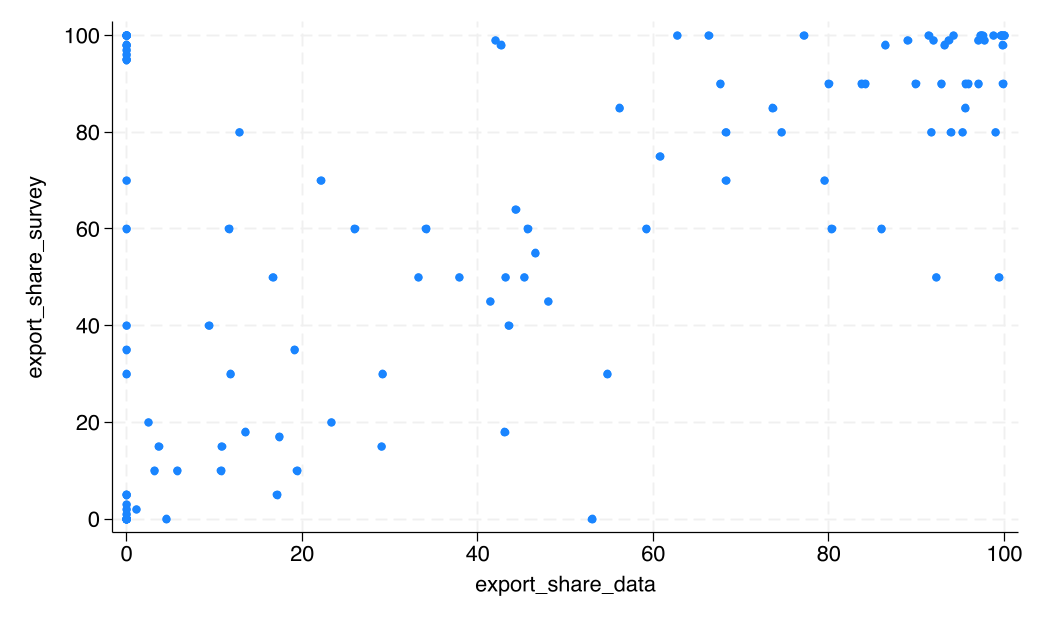
\includegraphics{fig/export_share_validation.png}
\end{frame}

\begin{frame}{Birth year of respondent and the CEO}
\protect\hypertarget{birth-year-of-respondent-and-the-ceo}{}
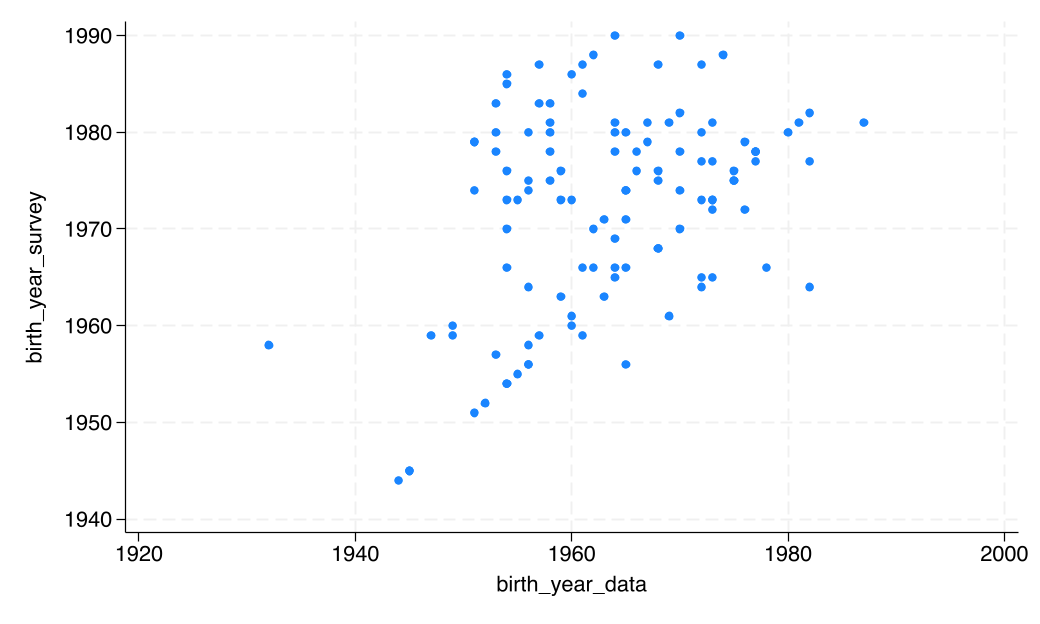
\includegraphics{fig/birth_year_validation.png}
\end{frame}

\begin{frame}{\ldots if the respondent \textbf{is} the CEO}
\protect\hypertarget{if-the-respondent-is-the-ceo}{}
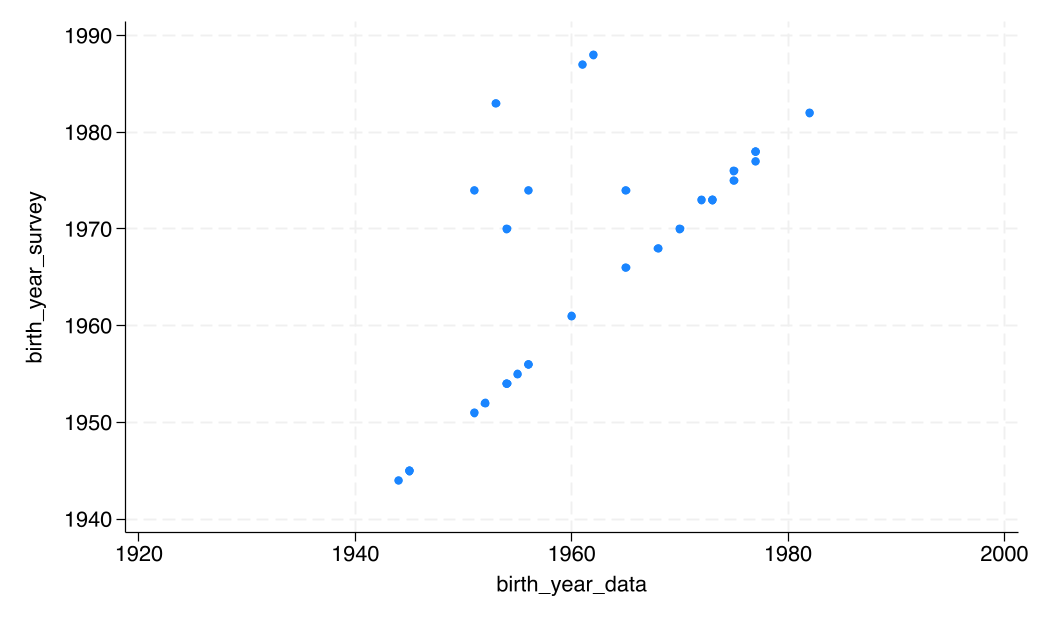
\includegraphics{fig/birth_year_validation_cleaned.png}
\end{frame}

\section{Management Scores}\label{management-scores}

\begin{frame}{Larger foreign firms are better managed}
\protect\hypertarget{larger-foreign-firms-are-better-managed}{}
\begin{center}
\begin{tabular}{lccc} \hline
 & (1) & (2) & (3) \\
VARIABLES & management & management & management \\ \hline
\vspace{4pt} & \begin{footnotesize}\end{footnotesize} & \begin{footnotesize}\end{footnotesize} & \begin{footnotesize}\end{footnotesize} \\
lnL & 0.455*** & 0.361*** & 0.326*** \\
\vspace{4pt} & \begin{footnotesize}(0.0593)\end{footnotesize} & \begin{footnotesize}(0.0589)\end{footnotesize} & \begin{footnotesize}(0.0665)\end{footnotesize} \\
foreign &  & 0.461*** & 0.437*** \\
\vspace{4pt} & \begin{footnotesize}\end{footnotesize} & \begin{footnotesize}(0.109)\end{footnotesize} & \begin{footnotesize}(0.111)\end{footnotesize} \\
exporter &  &  & 0.196 \\
\vspace{4pt} & \begin{footnotesize}\end{footnotesize} & \begin{footnotesize}\end{footnotesize} & \begin{footnotesize}(0.158)\end{footnotesize} \\
Constant & 0.568* & 0.856*** & 0.890*** \\
 & \begin{footnotesize}(0.318)\end{footnotesize} & \begin{footnotesize}(0.302)\end{footnotesize} & \begin{footnotesize}(0.306)\end{footnotesize} \\
\vspace{4pt} & \begin{footnotesize}\end{footnotesize} & \begin{footnotesize}\end{footnotesize} & \begin{footnotesize}\end{footnotesize} \\
Observations & 118 & 118 & 118 \\
 $R^2$ & 0.284 & 0.369 & 0.380 \\ \hline
\multicolumn{4}{c}{\begin{footnotesize} Robust standard errors in parentheses\end{footnotesize}} \\
\multicolumn{4}{c}{\begin{footnotesize} *** p$<$0.01, ** p$<$0.05, * p$<$0.1\end{footnotesize}} \\
\end{tabular}
\end{center}

\end{frame}

\section{Cohort Effects}\label{cohort-effects}

\begin{frame}{Older cohorts are worse managers}
\protect\hypertarget{older-cohorts-are-worse-managers}{}
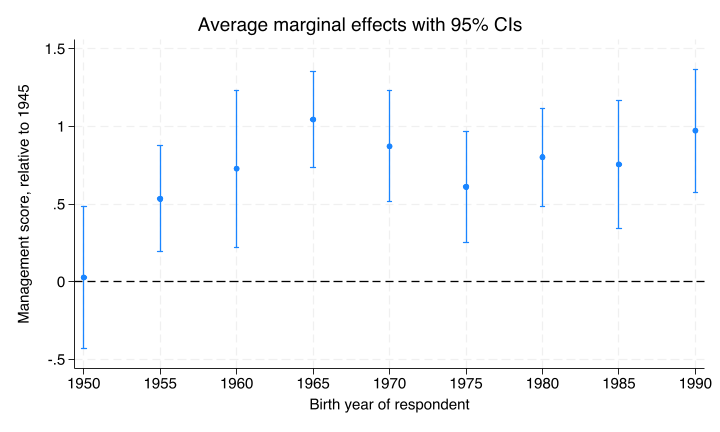
\includegraphics{fig/cohort-resp-marginsplot.png}
\end{frame}

\end{document}
